The safety and explainability of robotic systems has become increasingly important as applications for robotic systems transition to more unstructured and interactive environments. While one component to developing safe robots is to design robust and high-performing autonomy algorithms, another critical component is the analysis of the system's design. System analysis could come in several forms, including unit, component, or system-level testing, but one challenging aspect of testing is the determination of appropriate success criteria. It is also highly desirable to develop systems that are \textit{provably correct} or \textit{correct-by-construction} with respect to the stated success criteria.

This chapter introduces a set of rigorous mathematical tools and concepts for specifying desired behavior (i.e. requirements or specifications), proving that the system achieves the desired behavior, and synthesizing robot systems to be correct-by-construction. These mathematical tools are known as \textit{formal methods}\cite{ClarkeGrumbergEtAl2018}.

\notessection{Formal Methods}
Formal methods provide a mathematical framework for reasoning about a system's specifications as well as analyzing whether the system's behavior guarantees their satisfaction. Approaches for synthesizing provably correct behavior can also be built on top of these tools and are commonly incorporated within the umbrella of formal methods. Historically these techniques have been developed within the computer science community, and have been used to study problems related to logic, automatically proving properties of algorithms, checking the correctness of properties of circuits, and more. However in this chapter formal methods will be explored within the context of autonomous systems.

\begin{definition}[Formal Methods]
Formal methods are mathematically based techniques for the specification, development, and verification of software and hardware systems.
\end{definition}

It is important to note that formal methods are not just particular solutions or algorithms but rather are a class of tools and formalisms. Accordingly, this chapter will not focus on a particular algorithm (solution) for applying formal methods to problems in robotics, but will rather introduce several broadly used tools and techniques. Specifically, Section \ref{subsec:ltl} will introduce \textit{linear temporal logic}, which is a specialized language for writing specifications. Then the concept of the robotic system as a reactive model that can be \textit{verified} to satisfy the stated specifications will be introduced in Section \ref{subsec:verification}. Finally, the ability to \textit{synthesize} robot systems to provably be able to satisfy a specification will be explored in Section \ref{subsec:reactivesynth}.

\subsection{Linear Temporal Logic} \label{subsec:ltl}
Linear temporal logic (LTL) is a mathematical \textit{language} for formally expressing specifications or requirements on the system's behavior\footnote{Similar to how ordinary differential equations provide a mathematical ''language'' that is useful for modeling the kinematics and dynamics of physical systems.}. LTL is useful in robotics applications because it extends propositional logic\footnote{A formalism for expressing logical operations including conjunction (and), disjunction (or), and negation (not).} to handle \textit{temporal} components (assuming discrete time steps), which are common in sequential decision making problems and other robotics tasks. For example propositional logic can be used to write a specification that ``proposition $a$ and proposition $b$ must both be true'', while LTL extends the possible specifications to include temporal constraints such as ``proposition $a$ must be true \textit{until} proposition $b$ is true''.

The language of LTL can be expressed in terms of several atomic operators, the first few of which are inherited from propositional logic:
\begin{enumerate}
    \item \textit{true} or \textit{false} (Boolean values)\footnote{Technically false can also be written as $\lnot \text{true}$, where $\lnot$ is the ``not'' operator.} represent Boolean constants.
    \item $a$, $b$, $\dots$ (propositional symbols) denote single variables that can either be true or false at the current time step.
    \begin{figure}[ht]
    \begin{center}
    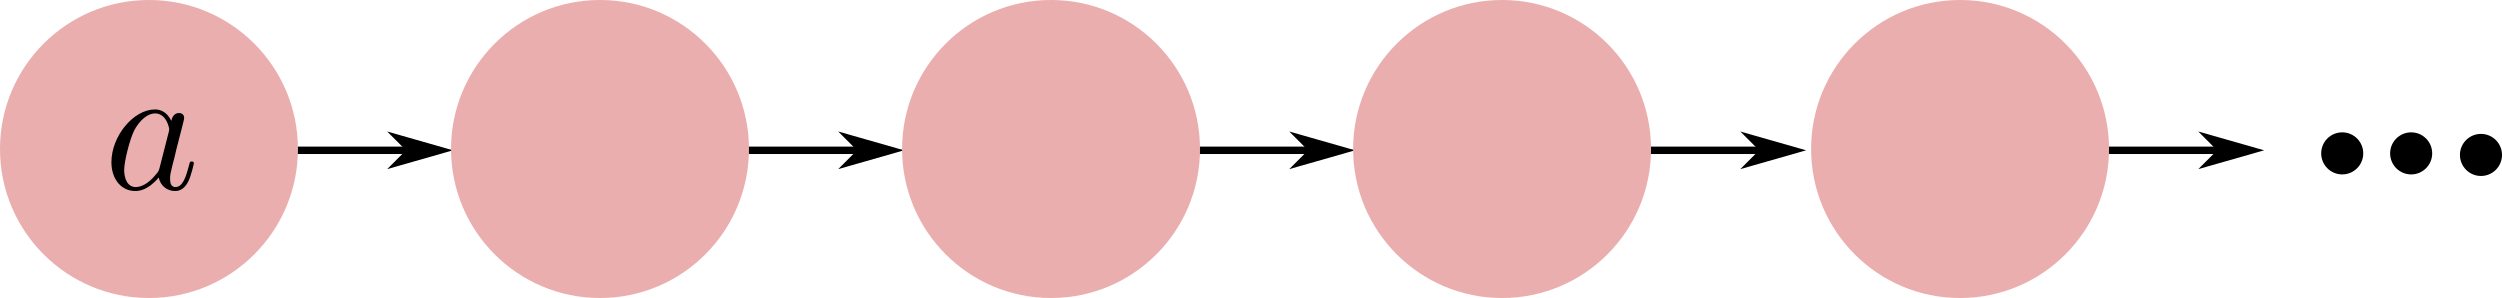
\includegraphics[width=0.5\textwidth]{tex/figs/ch25_figs/prop.png}
    \label{fig:propositionalvar}
    \end{center}
    \vspace{-\baselineskip}
    \end{figure}
    \item $\lnot \psi$ (negation operator\footnote{Technically \textit{false} can be written as $\lnot$\textit{true}.}) denotes the negation of $\psi$.
    \item $\psi_1 \land \psi_2$ (conjunction ``and'' operator) which can be read as ``$\psi_1$ and $\psi_2$''.
    \item $\psi_1 \lor \psi_2$ (disjunction ``or'' operator) which can be read as ``$\psi_1$ or $\psi_2$''. This operator can be expressed in terms of ``and'' and ``not'' as $\psi_1 \lor \psi_2 = \lnot(\lnot \psi_1 \land \lnot \psi_2)$.
    \item $\psi_1 \to \psi_2$ (implication operator) denotes that $\psi_1$ implies $\psi_2$. This operator can be expressed in terms of ``not` and ``or'' as $\psi_1 \to \psi_2 = \lnot \psi_1 \lor \psi_2$.
\end{enumerate}

Additional operators that are fundamental to LTL provide the capability for expressing temporal constraints:
\begin{enumerate}
\setcounter{enumi}{6}
    \item $X \psi$ (``next'' operator) denotes that $\psi$ happens next (at the next time step).
    \begin{figure}[ht]
    \begin{center}
    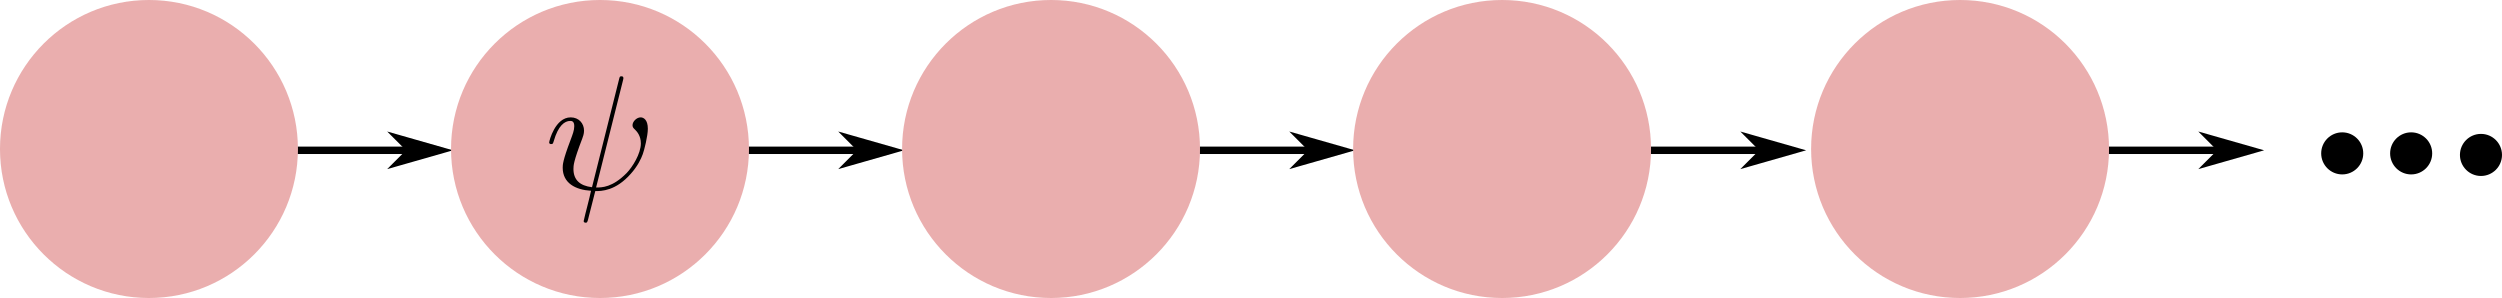
\includegraphics[width=0.5\textwidth]{tex/figs/ch25_figs/next.png}
    \label{fig:ltl_next}
    \end{center}
    \vspace{-\baselineskip}
    \end{figure}
    \item $\psi_1 U \psi_2$ (``until'' operator) denotes that $\psi_1$ should happen until $\psi_2$ happens.
    \begin{figure}[ht]
    \begin{center}
    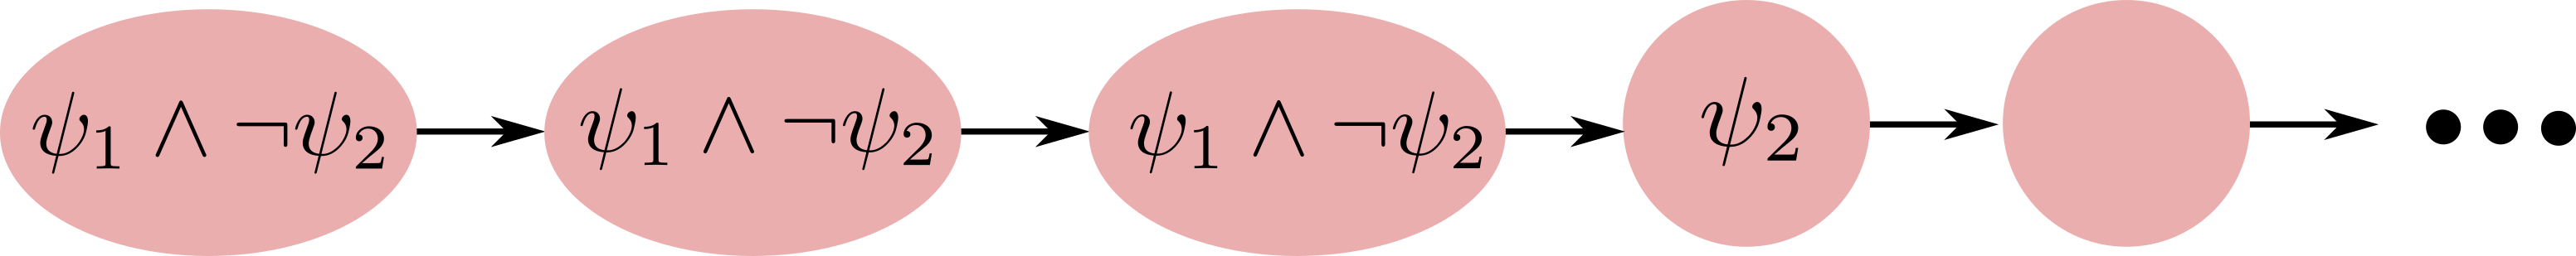
\includegraphics[width=0.65\textwidth]{tex/figs/ch25_figs/until.png}
    \label{fig:ltl_until}
    \end{center}
    \vspace{-\baselineskip}
    \end{figure}
    \item $F \psi$ (``eventually'' operator) denotes that $\psi$ happens at some point in the \textit{future}. This operator can be expressed in terms of the eventually operation as $F \psi = \text{true}\: U\: \psi$.
    \begin{figure}[ht]
    \begin{center}
    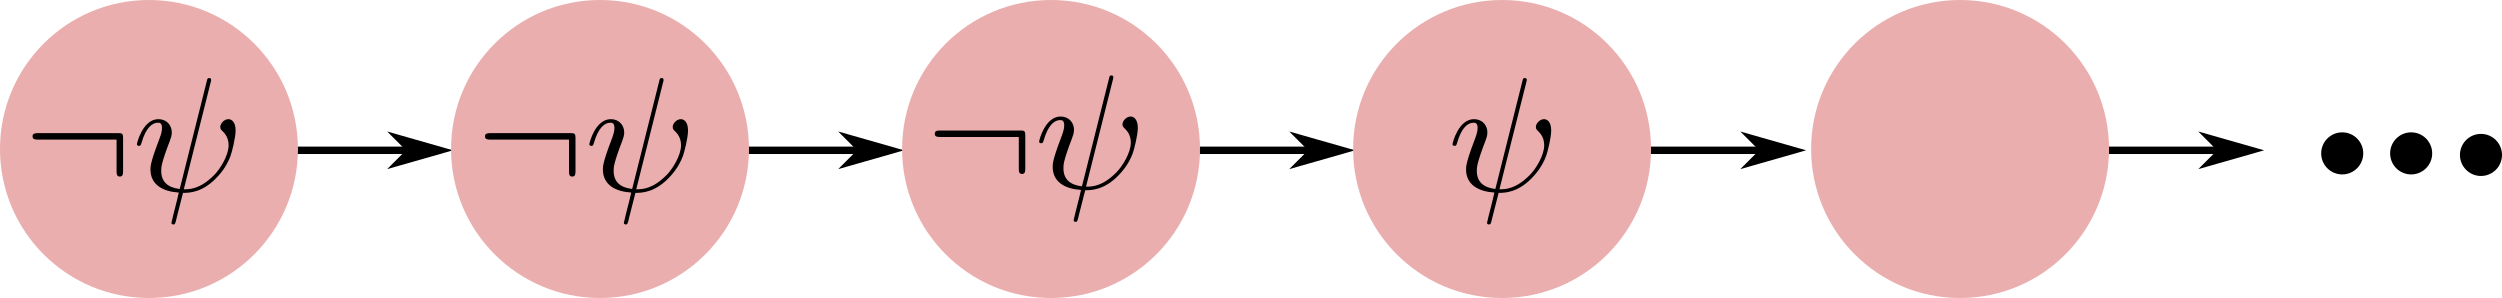
\includegraphics[width=0.5\textwidth]{tex/figs/ch25_figs/eventually.png}
    \label{fig:ltl_eventually}
    \end{center}
    \vspace{-\baselineskip}
    \end{figure}
    \item $G \psi$ (``always'' operator) denotes that $\psi$ happens globally (at all times). This operator can be expressed in terms of the negation and future operations as $G \psi = \lnot F {\lnot \psi}$.
    \begin{figure}[ht]
    \begin{center}
    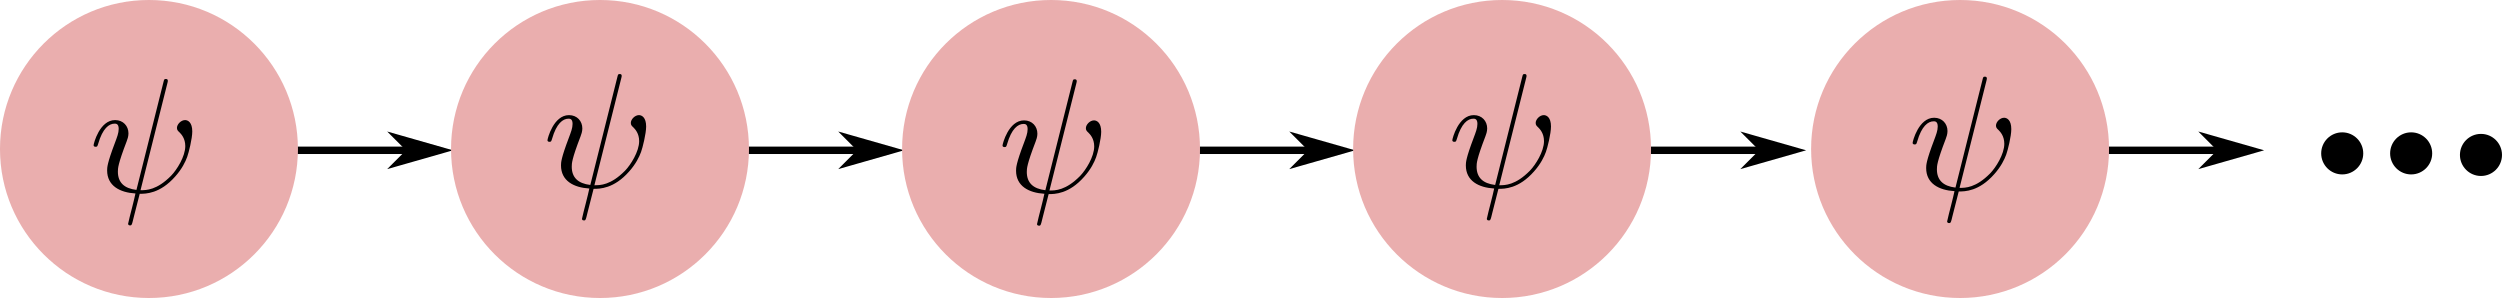
\includegraphics[width=0.5\textwidth]{tex/figs/ch25_figs/always.png}
    \label{fig:ltl_always}
    \end{center}
    \vspace{-\baselineskip}
    \end{figure}
\end{enumerate}
From these atomic operators it is possible to define many new specifications through \textit{composition}, and they can become arbitrarily complex as needed. A couple of common and useful compositions include:
\begin{enumerate}
\setcounter{enumi}{10}
    \item $GF \psi$ (``infinitely often'' composition) denotes that $\psi$ will eventually happen an infinite number of times (i.e. globally, $\psi$ will happen eventually). In other words there is always a $\psi$ in the future.
    \item $FG \psi$ (``stability''\footnote{This notion of stability is similar but not directly the same as the notions of stability from control theory.} composition) denotes that at some point in time $\psi$ will be true for all time thereafter (i.e. eventually $\psi$ will happen globally).
    \item $G(\psi_1 \to F\psi_2)$ (``response'' composition) denotes that for all time, whenever $\psi_1$ occurs then $\psi_2$ will occur sometime in the future. There are other useful variations on this composition, such as by replacing the $F$ operator with $X$ operator.
\end{enumerate}

Linear temporal logic provides a very powerful tool\footnote{There are also alternatives to LTL that provide even more powerful features, for example by not requiring a ``linear'' temporal structure but rather allowing for temporal ``branching''.} for abstractly talking about time, and in general the specifications written using LTL can in a way be more ``vague''. For example the eventually operator $F$ does not explicitly state \textit{when} something must occur, just that at \textit{some point} it will. It is also important to keep in mind that LTL is not an algorithm or technique for solving problems, but rather a language for \textit{formulating} problems (i.e. for expressing properties of interest such as system specifications). 

\begin{example}[Coffee Machine Specification] \label{ex:coffeespec}
Consider a simple robot that makes coffee. This robot has a button that a user can press, and has two functions: grinding coffee beans and brewing coffee. The desired behavior of this robot could be expressed by the designer as: \textit{if the start button is pressed, the robot will immediately start grinding beans for the next two cycles, and then brew the coffee for the next two cycles after that}. This specification, denoted as $\phi$, could be expressed via linear temporal logic as:
\begin{equation*}
\phi : G \big( \text{button} \to \text{grind} \land X \text{grind} \land XX (\lnot\text{grind} \land \text{brew}) \land XXX (\lnot\text{grind} \land\text{brew}) \big).
\end{equation*}
Note that the entire statement needs to be wrapped in the ``always'' operator to ensure this behavior can occur at any arbitrary time that a user presses the button.
\end{example}


\subsection{Verification} \label{subsec:verification}
System verification is the process of \textit{proving} that the system's behavior will satisfy the stated requirements and specifications (often expressed using linear temporal logic). In the terminology of formal methods, this system is typically referred to as the \textit{model}\footnote{The model could refer to a piece of software, a hardware component, an individual algorithm, or even an entire robot.} and the output of the verification\footnote{Also commonly referred to as \textit{model checking}.} procedure is a simple yes/no stating whether the model satisfies the specification. In this chapter the model will be denoted by $P$ and the specification by $\phi$, and the notation for stating that model $P$ satisfies specification $\phi$ is $P \models \phi$ (which can be read as ``$P$ models $\phi$'').

\begin{figure}[ht]
\begin{center}
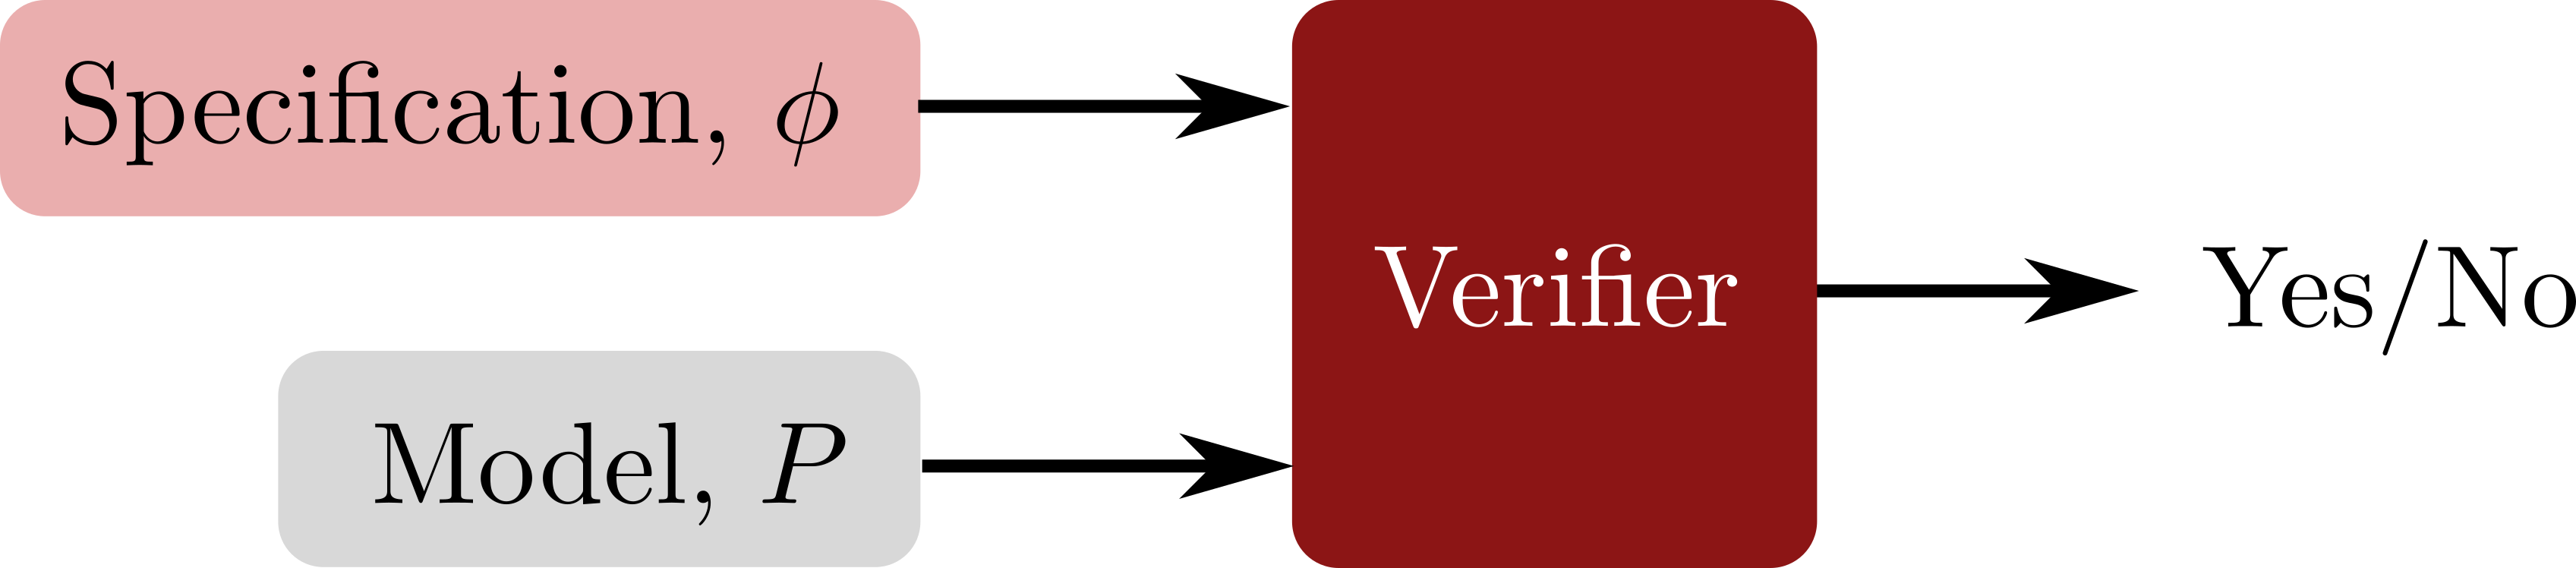
\includegraphics[width=0.65\textwidth]{tex/figs/ch25_figs/verification.png}
\caption{Given a system (model) and a specification, the process of verification proves whether the system satisfies the specification.}
\label{fig:verification}
\end{center}
\end{figure}

In this chapter it is assumed that the model $P$ is a \textit{reactive system}, meaning that its behavior is defined based on inputs $i$ which effect the system's outputs $o$\footnote{The inputs and outputs occur at each time step, and the behavior is assumed to be non-terminating.}. In contrast to robotic control problems where the ``inputs'' are generally the control inputs determined by the control algorithm, the inputs $i$ within this context refer to signals coming from the environment. The outputs $o$ of the model can then be thought of as the result of the system's decision making or underlying algorithm/process. As was mentioned previously, the model $P$ can take on many forms depending on whether the system is a hardware component, software component, algorithm, finite state machine, or even simply a mathematical function such as a machine learning model or control law.
\begin{marginfigure} 
\begin{center}
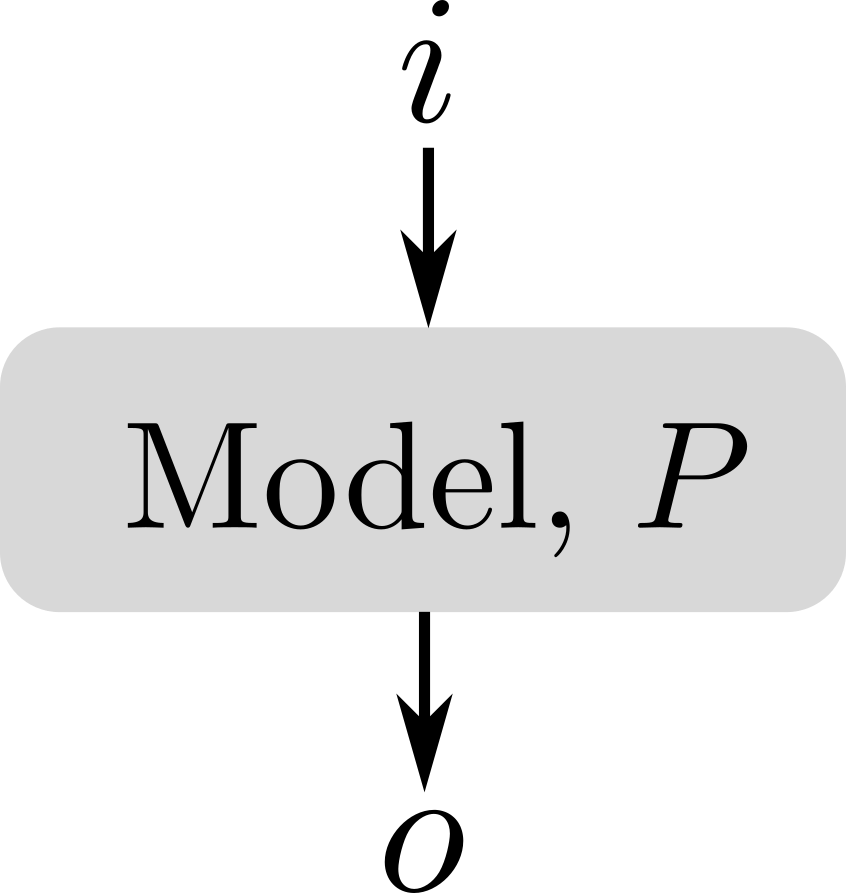
\includegraphics[width=0.5\textwidth]{tex/figs/ch25_figs/model.png}
\caption{The model $P$ is a system with inputs $i$ and outputs $o$. These inputs and outputs are used to express the model's specification $\phi$.}
\label{fig:reachtive_model}
\end{center}
\end{marginfigure}

For a given model $P$ the specification $\phi$ is assumed to be written in terms of the input and output sequences (i.e. the behavior is defined by the inputs and outputs of the system). Specifically, these sequences will be denoted as $\hat{i} = (i_0, i_1, \dots)$ and $\hat{o} = (o_0, o_1, \dots)$. With these definitions, the expression that $P$ satisfies $\phi$ can equivalently be written as $P \models \phi$ or $\hat{i} \cup \hat{o} \models \phi$. 

To summarize, the problem of model verification is to simply determine whether the input-output behavior of the model $P$ guarantees that $\phi$ is satisfied \textit{for all possible input sequences}.
There are several existing techniques that can perform system verification, and they may be tailored to the specific model form\cite{KwiatkowskaNormanEtAl2011}\cite{KatzHuangEtAl2019}.

\subsection{Reactive Synthesis} \label{subsec:reactivesynth}
Given a reactive model $P$ and a LTL specification $\phi$, the problem of verification is to determine whether the behavior of $P$ satisfies $\phi$ for all possible input sequences $\hat{i}$. But several important questions remain: how should the system be designed, and what should be changed if the verification step shows that $P \not \models \phi$? \textit{Reactive synthesis} addresses these problems by \textit{synthesizing} the system model $P$ to be correct-by-construction. In other words, in reactive synthesis the specification $\phi$ is first defined and then a model is constructed from scratch to satisfy the specification.
\begin{figure}[ht]
\begin{center}
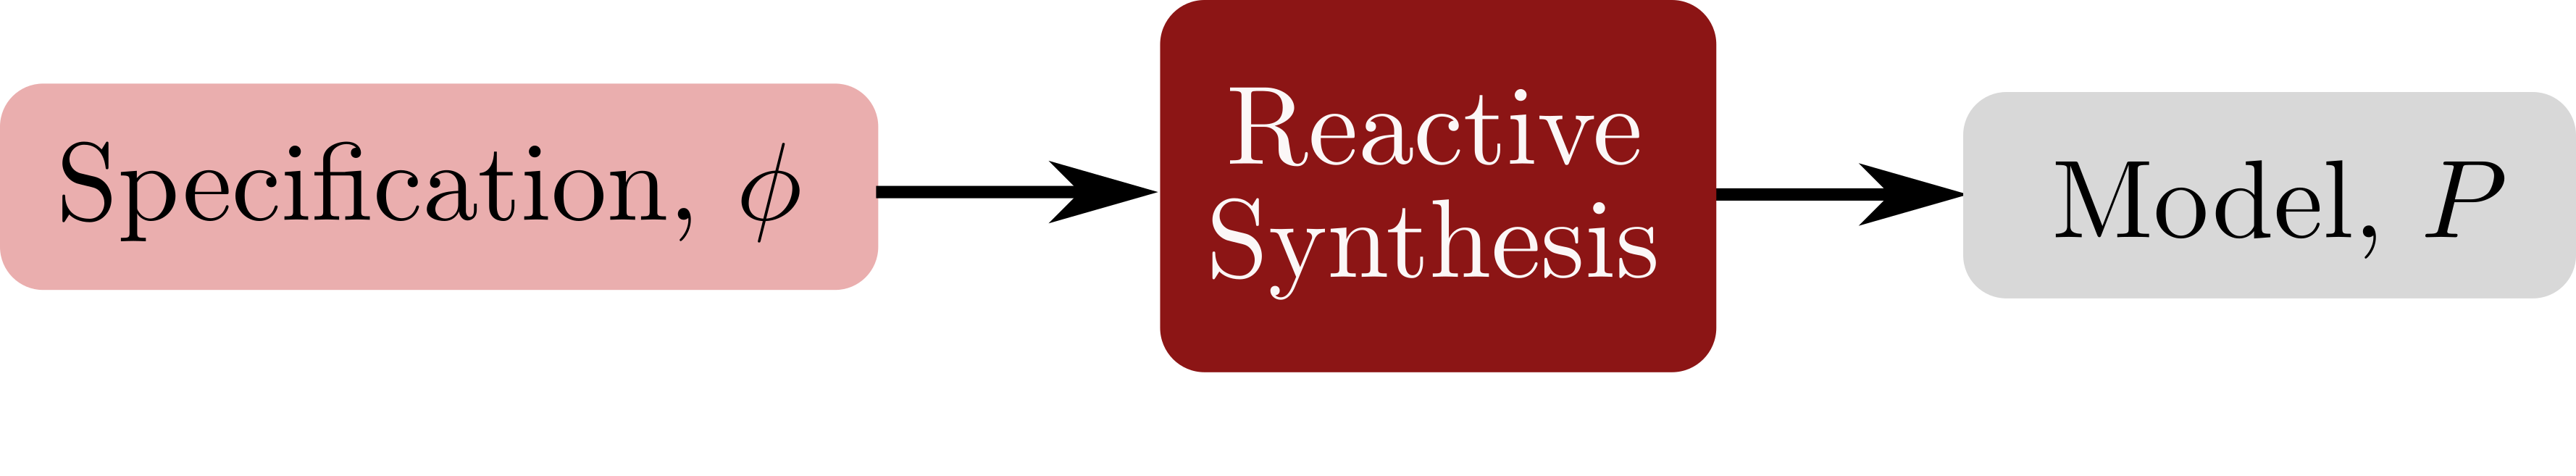
\includegraphics[width=0.65\textwidth]{tex/figs/ch25_figs/synthesis.png}
\caption{Given a specification $\phi$, the process of reactive synthesis generates a model $P$ that realizes the specification under all possible environmental inputs.}
\label{fig:formalmethod_synthesis}
\end{center}
\end{figure}

\subsubsection{Specification Satisfiability and Realizability}
The first step in reactive synthesis is to determine whether a model\footnote{Technically speaking, a \textit{finite state model}.} even exists which can satisfy the LTL specification $\phi$ for all possible input sequences. If no such model exists, then the system designer should reevaluate the specification itself.

In the nomenclature of formal methods, the specification $\phi$ is said to be \textit{realizable} if it can be satisfied for all possible input sequences, and it is \textit{satisfiable} if there exists at least one input sequence leading to satisfaction. These properties can be more rigorously defined in terms of the input and output sequences that describe the system's behavior:
\begin{definition}[Satisfiability]
A specification $\phi$ is \textit{satisfiable} if for some input sequence there exists an output sequence that satisfies the specification. Mathematically:
\begin{equation*}
\exists \: \hat{i} = (i_0, i_1, \dots), \quad \exists \: \hat{o} = (o_0, o_1, \dots), \quad s.t. \:\: \hat{i} \cup \hat{o} \models \phi.
\end{equation*}
\end{definition}
\begin{definition}[Realizability]
A specification $\phi$ is \textit{realizable} if for all possible input sequences there exists an output sequence that satisfies the specification. Mathematically:
\begin{equation*}
\forall \: \hat{i} = (i_0, i_1, \dots), \quad \exists \: \hat{o} = (o_0, o_1, \dots), \quad s.t. \:\: \hat{i} \cup \hat{o} \models \phi.
\end{equation*}
\end{definition}

Obviously the property of satisfiability is weaker than realizability, and realizability is much more important in practice. For example in order to guarantee safety in a rigorous way it is not sufficient to show that the system will be safe under a single scenario, but rather it should be shown for all scenarios. However, designing specifications that are realizable can be quite challenging, even in seemingly simple problems. As an example consider again the coffee machine robot from Example \ref{ex:coffeespec}.

\begin{example}[Coffee Machine Realizability]
The coffee machine robot from Example \ref{ex:coffeespec} had inputs $I = \{\text{button}\}$ and outputs $O = \{\text{grind}, \text{brew}\}$. For simplicity let $i_\text{button} = 1$ and $i_\text{button} = 0$ denote the button is pressed and not pressed, respectively. Additionally let $o_\text{grind}=1$ and $o_\text{brew}=1$ denote that the actions are occurring and let them be zero otherwise. 

Recall that the linear temporal logic specification for the robot's behavior was defined as:
\begin{equation*}
\phi : G \big( \text{button} \to \text{grind} \land X \text{grind} \land XX (\lnot\text{grind} \land \text{brew}) \land XXX (\lnot\text{grind} \land\text{brew}) \big).
\end{equation*}
This specification can now be analyzed to determine whether it is realizable. First, notice that one possible sequence of inputs and outputs that satisfies this specification is:
\begin{equation*}
\begin{split}
(i_\text{button}, \: o_\text{grind}, \: o_\text{brew})_k = \:&(0, \: 0, \: 0)_0, \\
&(1, \: 1, \: 0)_1, \\
&(0, \: 1, \: 0)_2, \\
&(0, \: 0, \: 1)_3, \\
&(0, \: 0, \: 1)_4, \\
&(0, \: 0, \: 0)_5, \\
& \quad\:\:\:\: \vdots
\end{split}
\end{equation*}
Because there exists a sequence that satisfies the specification $\phi$ it is by definition \textit{satisfiable}. However, consider a second input sequence $\hat{i} = (0, 1, 1, 0, 0, \dots)$ where the coffee machine's button is pressed twice in a row:
\begin{equation*}
\begin{split}
(i_\text{button}, \: o_\text{grind}, \: o_\text{brew})_k = \:&(0, \: 0, \: 0)_0, \\
&(1, \: 1, \: 0)_1, \\
&(1, \: 1, \: 0)_2, \\
&(0, \: ?, \: 1)_3, \\
\end{split}
\end{equation*}
At time step $k=3$ there is no combination of outputs that will satisfy the specification, since the first button press requires that $o_{\text{grind}, 3} = 0$ but the second button press requires that $o_{\text{grind}, 3} = 1$! Therefore by definition this specification is not \textit{realizable}\footnote{Does this mean it is impossible to automate a coffee maker? No! It just demonstrates that writing \textit{specifications} can be challenging.}.
\end{example}



\subsubsection{Synthesis for Realizable LTL Specifications}
If a LTL specification $\phi$ is realizable, then the synthesis problem seeks to find a finite state system that satisfies $\phi$ under all possible inputs. This can be accomplished by formulating the problem as a two-player game where the objective is for the system to generate ``winning'' outputs while the environment generates adversarial inputs. The two-player game formulation can be expressed mathematically by defining the following components:
\begin{enumerate}
    \item With the inputs $I$ and outputs $O$, at each time step the environment gets to choose from a set of $2^{\lvert I \rvert}$ actions and the system gets to choose from a set of $2^{\lvert O \rvert}$ actions.
    \item The strategy of the system is expressed as a function $f: (2^{\lvert I \rvert})^* \to 2^{\lvert O \rvert}$, where $f$ is a function from a finite sequence of environmental inputs to a specific output.
    \item The linear temporal logic specification $\phi$ is defined by the input and output sequences.
    \item The game is played for an infinitely long horizon, generating sequences $\hat{i} = (i_0, i_1, \dots)$ and $\hat{o} = (o_0, o_1, \dots)$.
    \item The game is won if $\hat{i} \cup \hat{o} \models \phi$.
\end{enumerate}

The process of converting a problem specification into this two-player game follows two main steps. First, the specification is converted into a \textit{non-deterministic B\"{u}chi automaton} and then the automaton is determinized to yield the game.
Once the game is appropriately formulated, it can be solved using existing algorithms to generate the policy $f$ that defines the system's behavior. Unfortunately, converting the specification into the automaton is computationally very challenging! In fact the computational complexity is \textit{doubly-exponential} in the size of the specification\footnote{A doubly exponential function has the form $f(x) = {a^b}^x$.}, which significantly limits the complexity of the problems that can be considered\footnote{This is one of the most significant limitations of formal methods in practical robotic settings, and approaches to overcome this complexity are still a topic of research.}. 

While the precise details for converting a specification into a two-player game and solving the game are beyond the scope of this chapter, the process can be explored visually through the following example.

\begin{example}[Simple Reactive Synthesis Problem] \label{ex:simplereactivesynth}
Consider the LTL specification $\phi: G(r \to X g)$ which states that whenever a request $r$ is received the system should provide a grant $g$ in the next time step. In this problem $I = \{r\}$ where $r$ denotes a request or no request and $O = \{g\}$ where $g$ specifies if a grant was made or not. The first step in transforming this specification into the two-player synthesis game is to generate the following B\"{u}chi automaton representation, as shown in Figure \ref{fig:automaton}.
\begin{figure}[ht]
\begin{center}
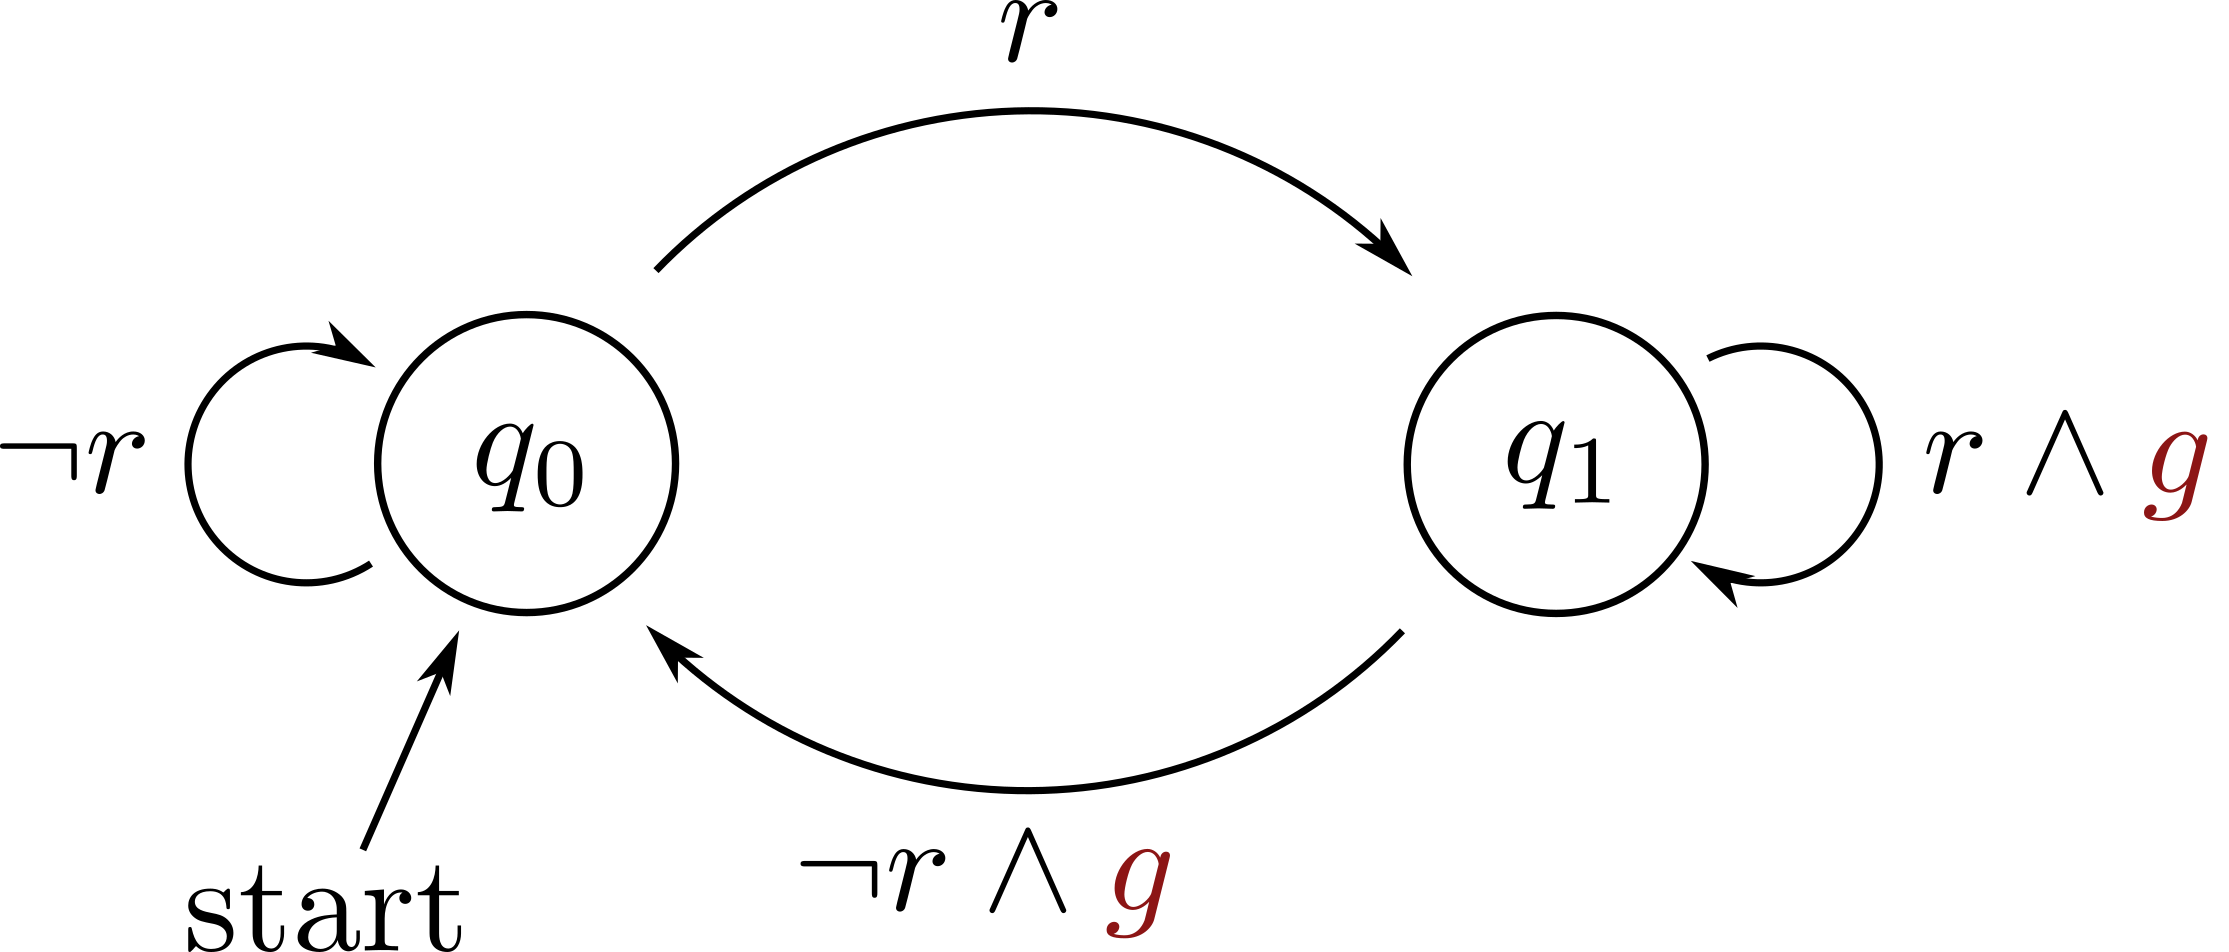
\includegraphics[width=0.55\textwidth]{tex/figs/ch25_figs/automaton.png}
\caption{The B\"{u}chi automaton representation of the LTL specification $\phi: G(r \to X g)$.}
\label{fig:automaton}
\end{center}
\end{figure}
In Figure \ref{fig:automaton} the variables $q_0$ and $q_1$ represent states of the automaton, and the transitions between the states are dependent on the environmental inputs and the system's behavior.

The two-player game is generated from this B\"{u}chi automaton\footnote{This automaton is already deterministic, so no determinizing step is needed.} by introducing intermediate states as well as the unsafe ``contradiction'' state (denoted in Figure \ref{fig:synthesis_2pgame} as $\bot$). This game is represented graphically in Figure \ref{fig:synthesis_2pgame} where the $*$ denotes that any action could be taken by the model and the small grey circles represent the intermediate states.
\begin{figure}[ht]
\begin{center}
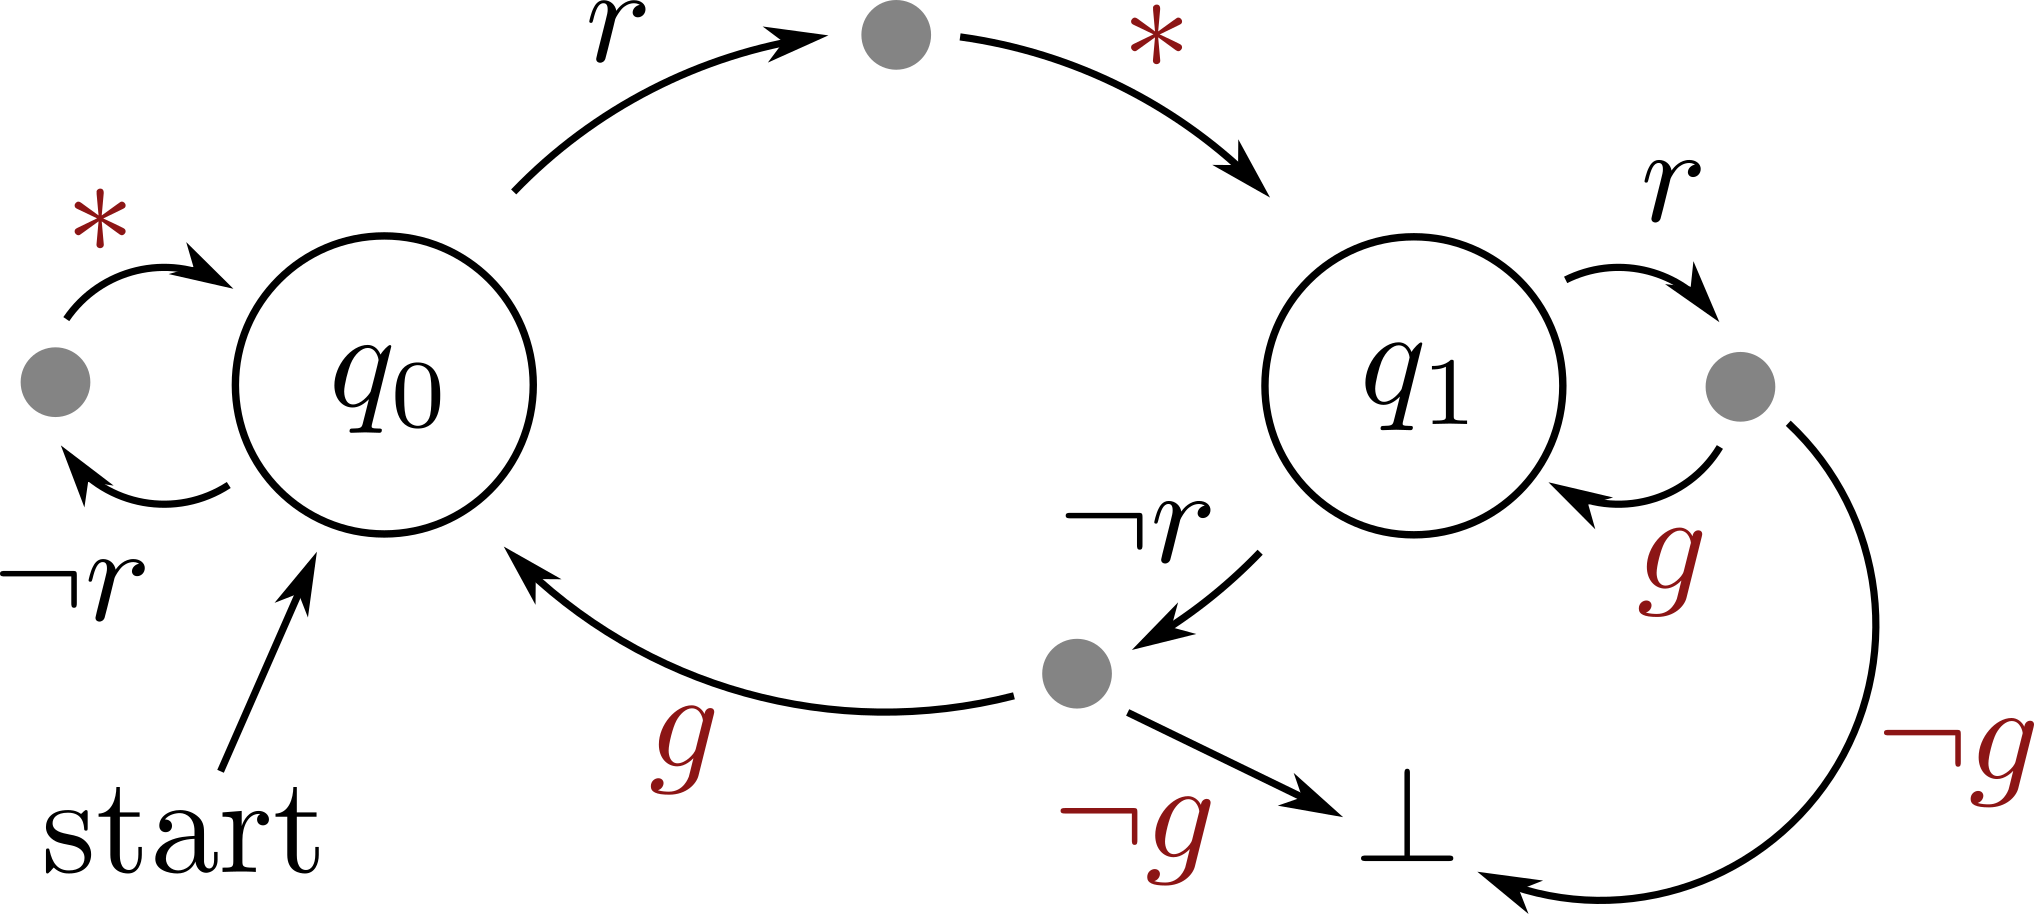
\includegraphics[width=0.5\textwidth]{tex/figs/ch25_figs/game.png}
\caption{The two-player game representation derived from the B\"{u}chi automaton in Figure \ref{fig:automaton}.}
\label{fig:synthesis_2pgame}
\end{center}
\end{figure}
The system can ``win'' this two-player game by ensuring that the contradiction state is never reached, which then defines the system's behavior! By analyzing Figure \ref{fig:synthesis_2pgame}, it turns out that one ``winning'' strategy strategy (behavior) is for the system to \textit{always} provide a grant! This strategy is shown graphically in Figure \ref{fig:synthesis_2pgamesol}.
\begin{figure}[ht]
\begin{center}
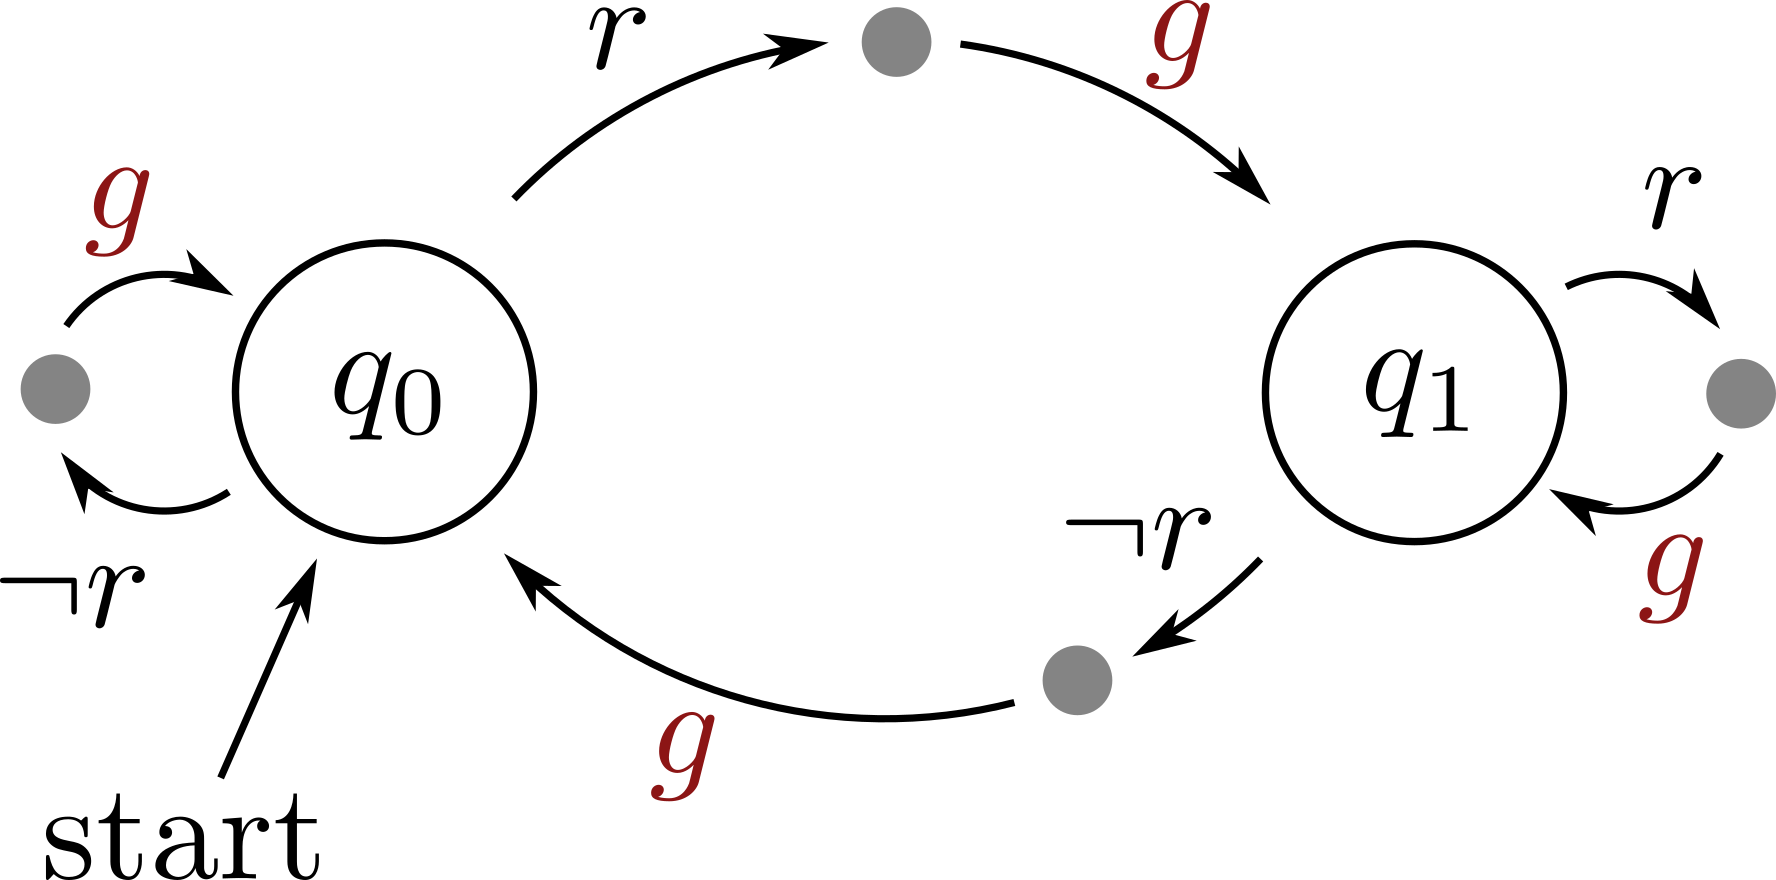
\includegraphics[width=0.45\textwidth]{tex/figs/ch25_figs/game_solution.png}
\caption{A strategy for the system in Example \ref{ex:simplereactivesynth} to ensure the specification is met is to \textit{always} provide grants, which is guaranteed to avoid the contradiction state in the two-player game shown in Figure \ref{fig:synthesis_2pgame}.}
\label{fig:synthesis_2pgamesol}
\end{center}
\end{figure}
\end{example}